
为了更好理解制度变化

在基于主体的模型(Agent-based Model, ABM)中,主体的行为都是在一个由斑块组成的“世界”内进行的。这个世界中不同的斑块可能具有一些属性上的本质差异。
此外,在处理实际问题时,我们需要常常是一块形状不规则的地图。这类似于一个多个属性、多个图层的斑块组合。能够从不同的文件输入中提取出这些属性组合将有助于模型的实际应用。

\begin{figure}[htb]
    \centering
    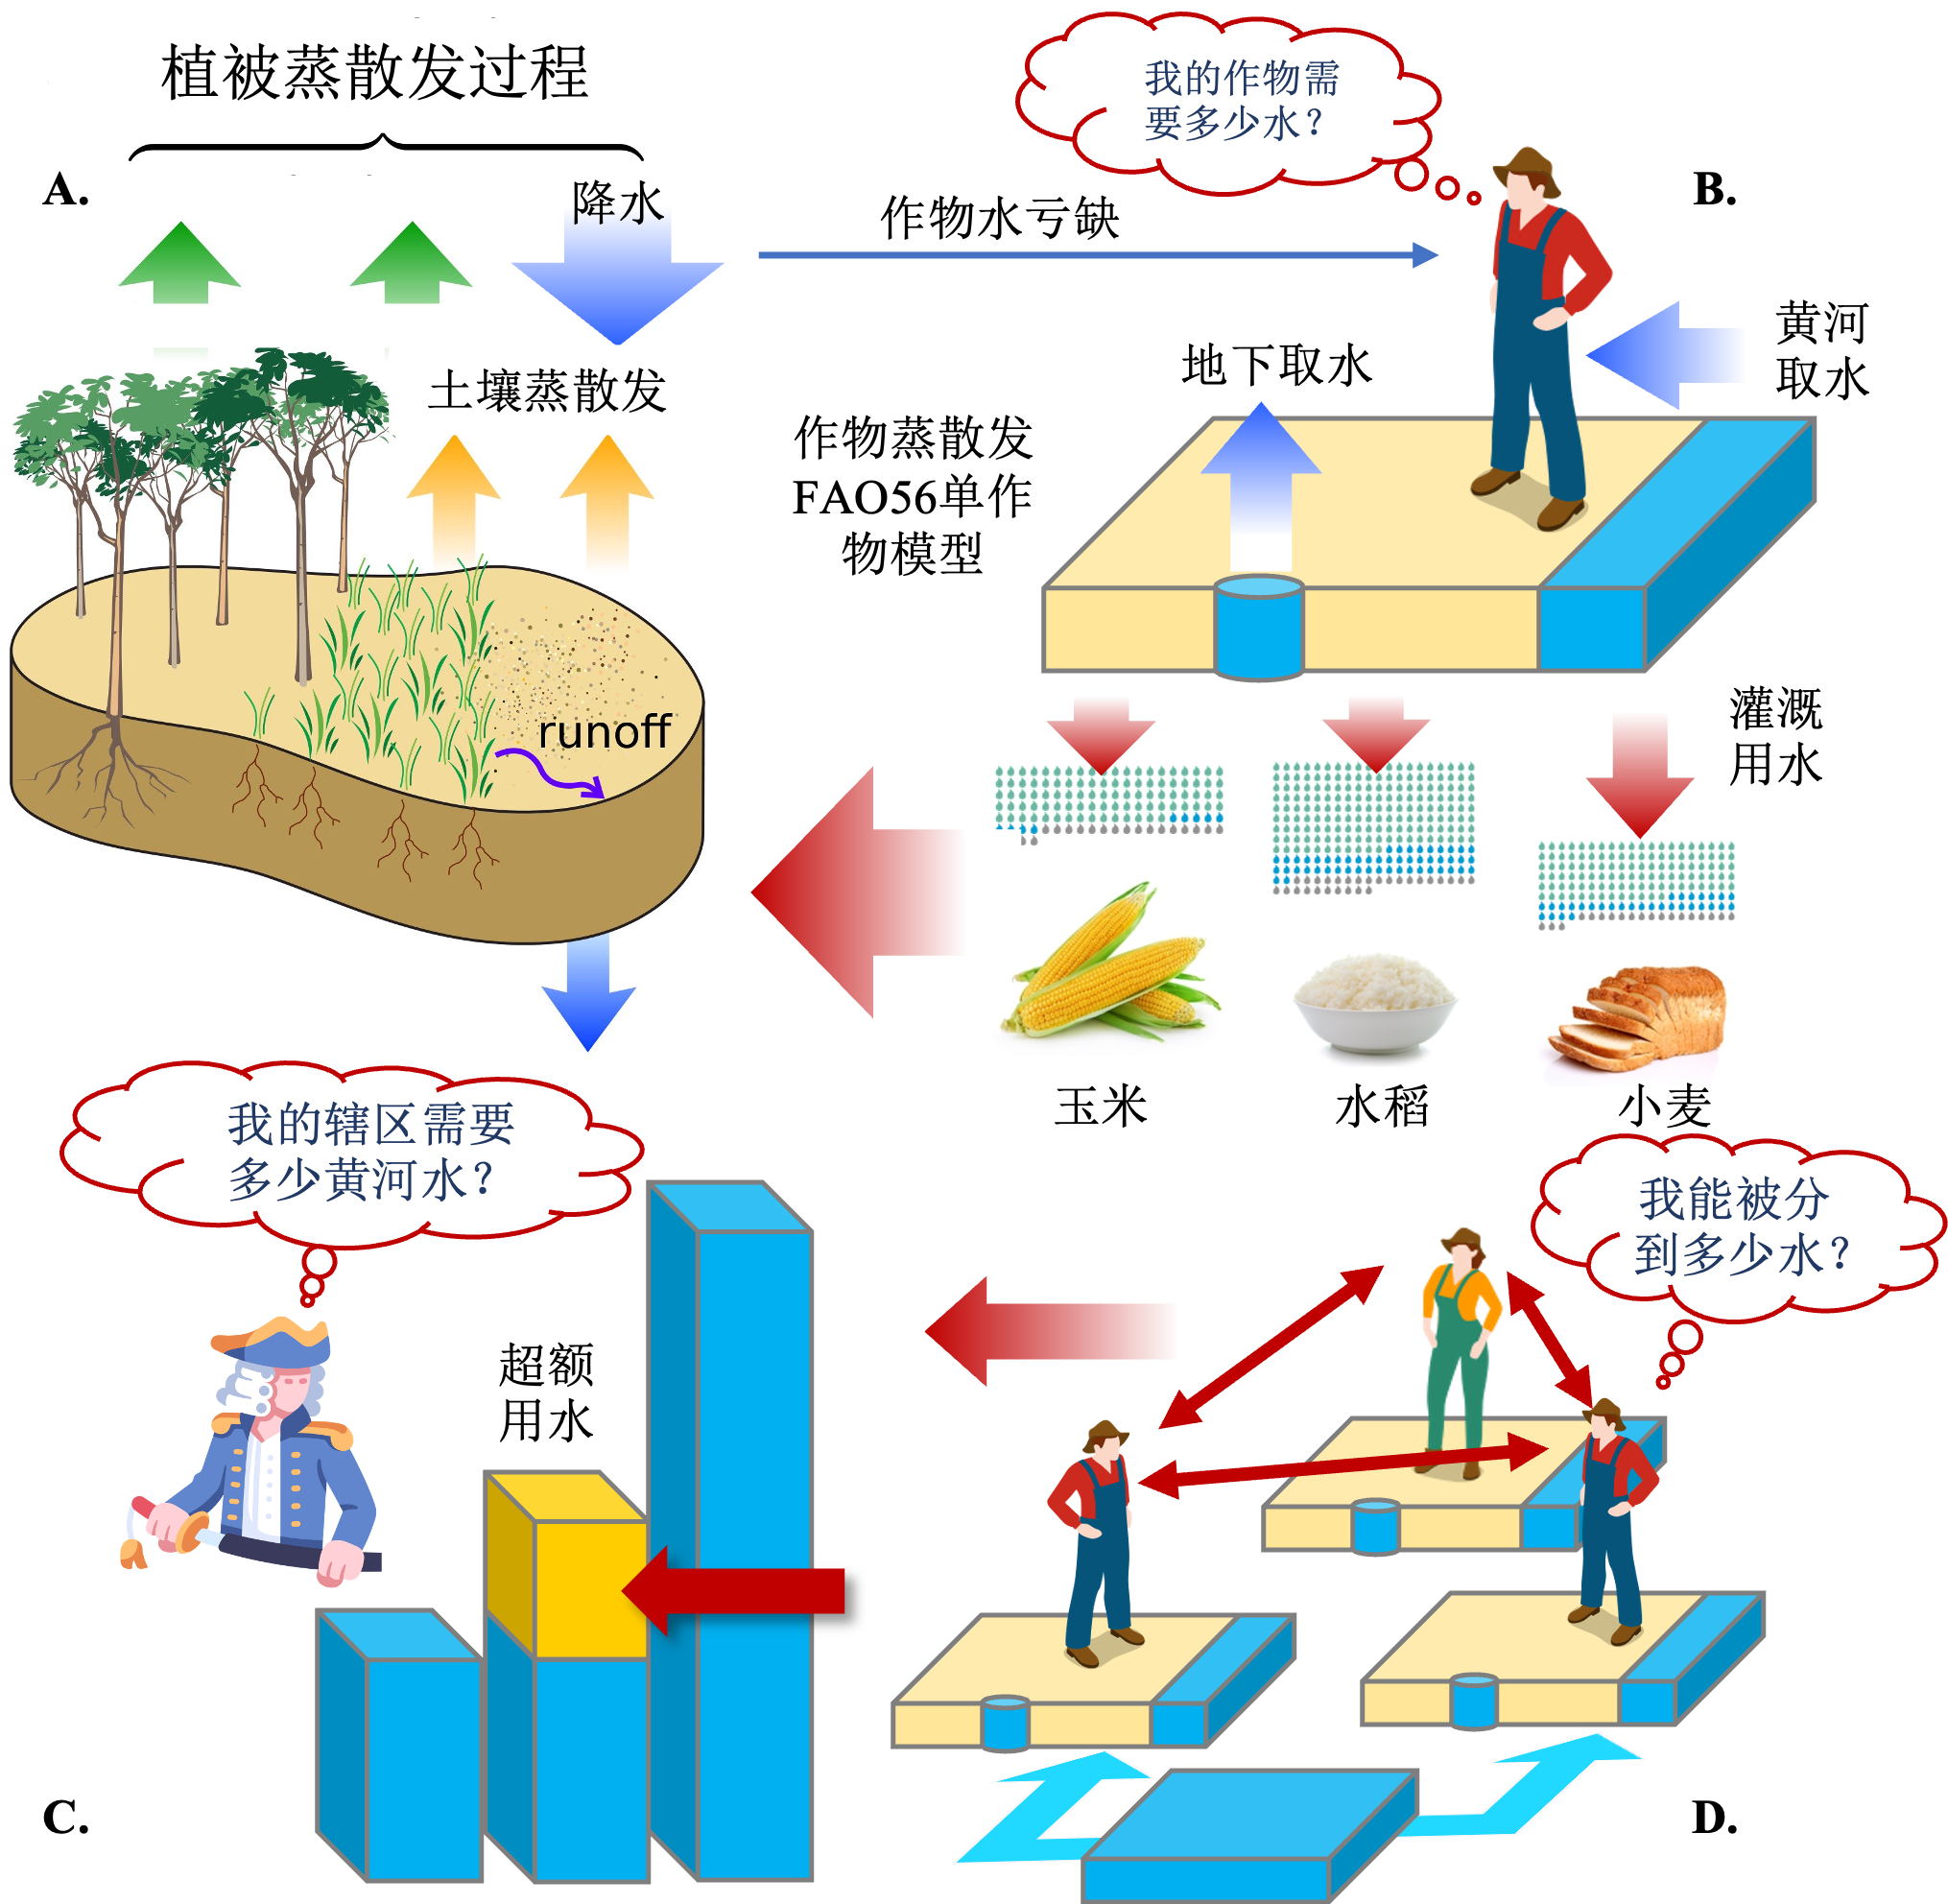
\includegraphics[width=\textwidth]{img/ch6/ch6_framework.png}
    \caption{多主体模型设计框架}\label{ch6:fig:framework}
\end{figure}

\subsubsection*{个体尺度}

\subsubsection*{社区尺度}

\subsubsection*{地区尺度}

\subsection{模型框架介绍}

虽然多主体模型适用于基于规则的模拟,但它通常会过度简化空间信息,从而使模型变得抽象。针对这个问题,本研究开发了基于地理数据的多主体建模框架“ABSESpy”。这个框架使用真实的地理空间数据集来构建人工社会生态系统,同时充分考虑人类行为因素。它支持使用地理数据代理,如Shapefile、GeoTiff和NetCDF等,在建模环境中,对具有认知、传染和反应等行为的代理人进行建模。该框架可以调度任意数量的自然模块和社会模块,并使它们之间松散耦合。这意味着用户可以专注于分别实现人类行为的逻辑和自然过程的仿真,该框架使得两者之间能够安全、轻松地查找、访问和修改值。因此,使用ABSESpy框架可以更准确地模拟社会-生态系统,同时也能更好地解决空间信息过度简化的问题。

\subsection{社会模块}

个体能够利用他们的主观能动性来做出决定,所以微观个体可能会对某些社会生态环境做出不同的反应。然而,在某种文化规范下,一些反应因为符合社会规范而受到奖励,而另一些反应则因为背离社会规范而受到惩罚。这种深刻的影响塑造了它们在资源进化博弈中的社会学习过程。

这个模块提供了一些函数来测量代理如何因为这些对齐/不对齐而保持或失去社会匹配。
这一过程基于多元理性(Plural rationality theory PRA)的社会理论,这是一个理解个人决策与社会规范影响之间关系的经典框架。多元理性方法框架已被应用于解释水治理的成功与失败。  % TODO citation

多元理性理论可以对复杂的政策问题进行了结构化的诊断,已被运用于。
这个框架指出,任何社会领域都由四种生活方式的动态组合和再创造组成,即等级制度、平等主义、个人主义和宿命论。每种生活方式都包括组织社会关系的特定模式,以及相应的文化偏见。这个理论认为,如果人类文化呈现出丰富的多样性,那是因为指数级的文化形式可以从有限的选择中产生出多种组合 [@verweij2015]。

% Cobb-Douglas函数(https://inomics.com/terms/cobb-douglas-production-function-1456726)
社会得分是一个Cobb-Douglas函数,在福利经济学中常用的,例如幸福指数和人类发展指数。
% [Happy Planet Index](https://happyplanetindex.org/) 
% 人类发展指数(http://hdr.undp.org/en)

考虑到人们不愿意主动得罪别人,也不愿意丧失名誉,我们采用的函数形式是:

\begin{equation}
    S = {(grid)}^m * {(1 - group)}^n
    \label{ch6:eq:society}
\end{equation}

其中 $m$ 是一个农民报告邻居违规用水的次数,$n$ 则是他被报告违规用水的次数,因此:

- $grid^m$ 这部分表达的是一个 Agent 得罪人而感到不舒服
- $group^n$ 这部分表达的是一个 Agent 因为违规被周围人指指点点而感到不舒服

这个社会效用函数在过往的研究中也有使用,如 Castilla-Rho et al., (2017, 2019) [@castilla-rho2017, @castilla-rho2019]. 如果没有指定这两个参数,我们将参考 [@castilla-rho2017] 的研究从数据库中直接为这两个参数指定值。
这个社会效用函数的参数(Grid 和 Group)可以用各个地区的文化差异来进行量化:

% ![CleanShot2022-08-15at08.57.49@2x](https://songshgeo-picgo-1302043007.cos.ap-beijing.myqcloud.com/uPic/CleanShot%202022-08-15%20at%2008.57.49@2x.png)

\subsection{水平衡模块}

\subsection{数据处理}

作物物候、气象、灌溉强度、灌溉面积、用水配额等

模型能够模拟各省份绿水(降水+土壤水)/蓝水(地表/地下水)的使用情况
